\documentclass[a4paper]{article}

% Packages{{{
  \usepackage[margin=1in]{geometry}                           % Margins
    \linespread{1.2}                                          % Increases line spacing
  \usepackage{graphicx}                                       % Image Support
    \graphicspath{ {./images/} }                              % Path to image directory
  \usepackage{color}                                          % Colors for stuff
  \usepackage[dvipsnames]{xcolor}                             % Extra-Colors
  \usepackage{soul}                                           % Provides Highlight feature
  \usepackage{todonotes} 
  \usepackage{fancyhdr}                                       % Fancy Header and footer
  \usepackage{amsmath}                                        % Math support
  \usepackage{amssymb}                                        % Extended symbols for math
  \usepackage{listings}                                       % Code-snippet support
  \usepackage{caption}                                      % Caption support
  \usepackage[utf8]{inputenc}                               % utf encoding
  \usepackage{hyperref}
    \hypersetup{pdfnewwindow=true, colorlinks=false}
%}}}

% Footer section {{{
  % Creates footer
  \pagestyle{fancy}%
  \fancyhf{}%
  \lfoot{Swapnil}%
  \cfoot{iamb4uc.xyz}%
  \rfoot{Page \thepage}%
  \renewcommand{\headrulewidth}{0pt}% Line at the head invisible
  \renewcommand{\footrulewidth}{0.4pt}% Line at the footer visible

  % Redefine the plain page style for chapter pages
  \fancypagestyle{plain}{%
    \fancyhf{}%
    \fancyfoot[L]{Swapnil}%
    \fancyfoot[C]{iamb4uc.xyz}%
    \fancyfoot[R]{Page \thepage}%
    \renewcommand{\headrulewidth}{0pt}% Line at the head invisible
    \renewcommand{\footrulewidth}{0.4pt}% Line at the footer visible
  }
% }}}

% Title {{{
  \title{\Huge{\emph{Management Information System}
  }
  }
\usepackage{blindtext}
  \author{\huge{by \emph{Swapnil}}\\ \\ \Large{written in {\LaTeX}}
  }
  \date{\today}
% }}}

\begin{document}
%Title page{{{
  \maketitle
  \thispagestyle{empty}
%}}}

% ToC{{{
  \setcounter{tocdepth}{3}
  \tableofcontents
  \newpage
%}}}
% -----------------------------------------------------------------------------

\part{TODO}
\section{Business Process reengineering}

\part{Everything Else}
\section{How does Modern Business influence Information Systems?}
With the constant change and evolution of customer preferences and requirements
– businesses that can bring about new methods and innovative techniques can
survive the market and continue to function as per the customer demands. The
implementation of information system can benefit a lot in businesses and helps
in controlling the internal and external processes.

Following are the benefits of information system
\begin{enumerate}
  \item \textbf{New Products and Services}

    Any business striving to enhance and to give a strong hold on the future
    has to instill a well organized Business Information System. An IS can
    help in analyzing independent processes and enables organized work
    activities. Hence an information system entitles the companies to
    understand how the company generates, develops and sells the services or
    products.

  \item \textbf{Information Storage}

    Keeping a log of activities is important for all the organizations, to
    understand the reason for the problems and so to provide solution to the
    same. Business Information System makes it simple to store operational
    data, revision histories, communication records and documents. The storing
    of data manually involves a lot of time and money. A sophisticated
    Information system stores the information in the database which simplifies
    the process of finding the data easily.

  \item \textbf{Simplified Decision Making}

    Business Information System, eases the process of decision making and
    simplifies the process of delivering the required information and hence
    assists in taking better decisions instantly.

  \item \textbf{Behavioral Change}

    Business Information System can be effectively implemented to help
    communication better between the employers and the employees. Information
    Systems work better as it stores documents and files in folders that can
    be accessed and shared by the employees. This ensures to oversee the flow
    of information between the management and the lower-level employees. This
    also allows the front-line employees to be a part of the decision
    making process and hence feel motivated and committed towards doing a task.
\end{enumerate}

\section{Difference between Transaction Processing System and Management
Information System}
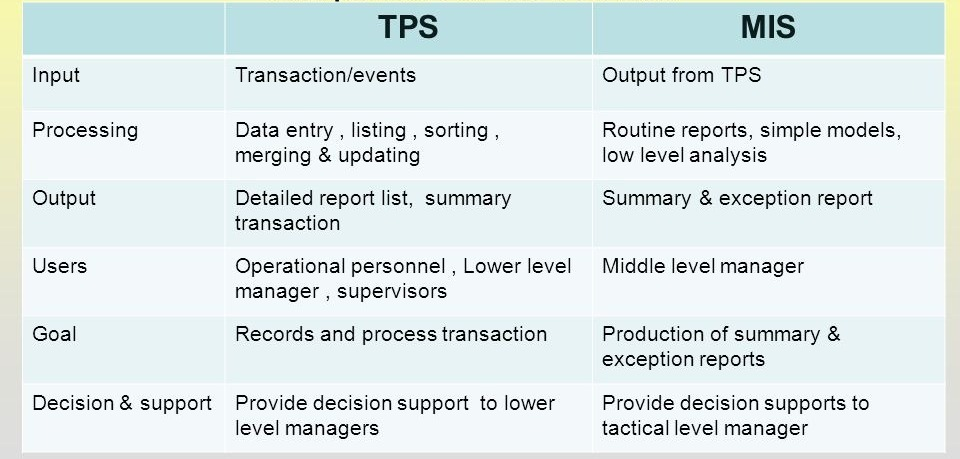
\includegraphics[scale=0.4]{difftpsmis}

\section{Application of database in business\\
\emph{or} \\ 
Uses of database management system in business}
With DBMS, businesses can increase their access to data and help end users
throughout the organizations share the data. As a result, these end users can
deliver faster sales and make quicker decisions as they have access to the
exact data they need.

\begin{enumerate}
  \item \textbf{Customer Relationship Management}

    A customer relationship management (CRM) database can help a small business
    manage the lifeblood of its business – its customers. A CRM database
    organizes all the information a company has about its accounts, contacts,
    leads and opportunities.


  \item \textbf{Inventory Tracking Database}

    An inventory tracking database can tell a retail business how much
    inventory is in a warehouse, in a storage room and on store shelves.


  \item \textbf{Payroll and Scheduling Database}

    Using a database to manage employee information can simplify scheduling and
    help prevent payroll errors. An employee database contains such fields as
    hourly wage, salary or commission, tax withholding rates, year-to-date
    income and accrued vacation time.


  \item \textbf{Business Data Analysis}

    The robust reporting features of databases make them useful resources
    for analyzing data and predicting future trends.
\end{enumerate}

\section{E-commerce}
Few concepts have revolutionized business more profoundly than e-commerce.
E-commerce is changing the shape of competition, speed of action and the stream
lining of interactions to companies and from companies to support.

\section{E-business}
Electronic business is any kind of business or commercial transaction that
includes sharing information across the internet. Commerce constitutes the
exchange of products and services between businesses, groups, and
individuals and can be seen as one of the essential activities of any
business.


\section{Difference between e-commerce and e-business}
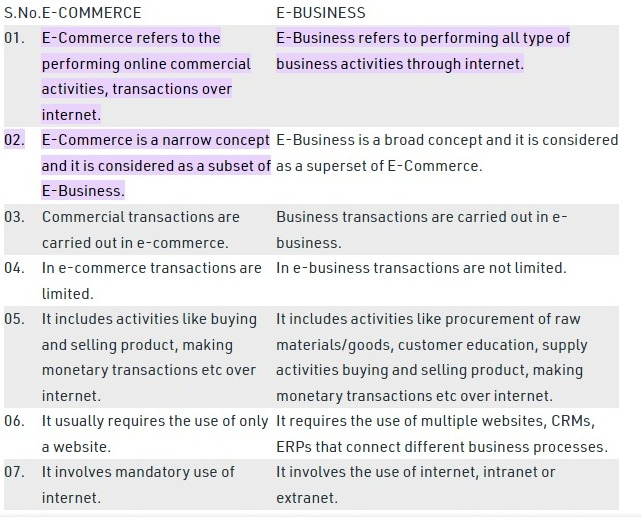
\includegraphics[scale=0.7]{diffecomebuis}

\part{Unit 2}
\section{Different IT tools used to grow business.}
\subsection{IT applications used in business.}
There are 7 types of business technology tools to save time and money 

\begin{enumerate}
\item Task Management Tools.
\item Email and Social Marketing.
\item Social Media Scheduling Tools.
\item Scheduling Meetings.
\item Obtaining e-Signatures.
\item Finding and Retaining Business Clients.
\item Document Collaboration.
\end{enumerate}
\section{Difference between inter and extranet}
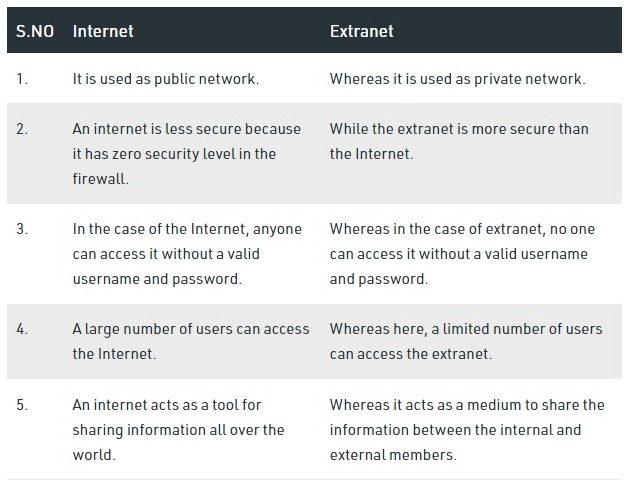
\includegraphics[scale=0.7]{diffinterextra}

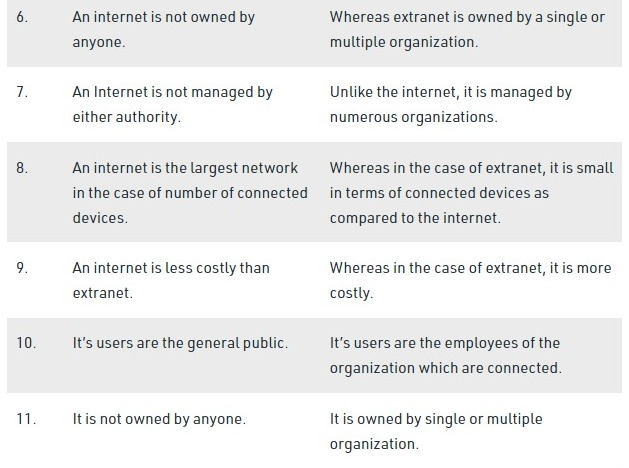
\includegraphics[scale=0.69]{diffinterextra2}

\section{Advantages of E-commerce}
There are various benefits of E-commerce to consumers that are listed as
follows

\begin{enumerate}
  \item It is also mentioned in features of e-commerce that it provides
    24x7 supports to its consumers. It provides the facility of placing
    orders anytime, anywhere, or from any location.
  \item It provides more options to its customers and gives a faster
    delivery of products.
  \item Users can select cheaper and better options via e-commerce as it
    provides more options to its customers.
  \item Before the final purchase of a product, a customer can see the
    reviews and comments of a particular product and can also put their
    reviews and comments about a product.
  \item It provides the information in an easy way, i.e., the information
    is not hard to read. A customer can see the…
\end{enumerate}

\section{Disadvantages/drawbacks of E-commerce}
The limitations of using e-commerce are mentioned as follows

\begin{enumerate}
  \item As there is a requirement of the internet to use e-commerce, it is possible that the internet may be slow.
  \item It does not have any universal standard for reliability and quality.
  \item There can be compatibility issues.
  \item Security is another concern of using e-commerce. We have seen security breaches many times where the customer's information got stolen. Some of the big concerns with customers include identity theft, credit card theft, etc.
  \item E-commerce uses a public key that is not secure.
  \item It is a major drawback in E-commerce that there is a lack of feel or touch of products while purchasing them online.
  \item It is inconvenient to use the internet for those people who are living in remote villages, and it is still not cheaper.
\end{enumerate}

\section{MIS of school management system and college management system}
The present education structure is radical, open and more practical. The
days are gone when school and colleges were loaded with files and other
paper-based record books. Thanks to the school management system software
that completes arrays of tasks including the student’s fee, the teacher’s
salary, attendance register, timetables for all classes, fee records,
examination records and results of the exams within no time.

There are many reasons why an increasing number of schools are using school
management software on regular basis.
\begin{enumerate}
  \item Easy Communication 

    Best school software helps a school communicate in an effective way
    with the parents. The school management find easy in sharing
    information and circulating. All the communication relevant tasks are
    done in short span of time and more effectively. Parents can check
    result of their child online. Undoubtedly, this software has
    strengthened the participation and communication of parents with
    school. Schools can focus more on efficient education delivery as
    tedious clerical operations are taken care by ERP software.

  \item HR \& Payroll Management System

    Every school keeps a systematic and easy approach towards maintaining
    and updating the different aspects of their institute. School ERP
    online gives comprehensive reports related to employee’s data,
    attendance, salary, leave, increments, da-arrear, bonus, tax
    calculation and many more. Even it gives a go-ahead formula builder to
    customize salary structure as per school’s need.

  \item Library Management

    An institution with big library needs to be maintained properly and
    preserved carefully year after year. They need enough space to store
    and have to be protected from natural hazards like rain and fire etc.
    But with the use of school management system software, it’s easy to
    preserve records on PC for many years. The software manages all data
    related to library including record of issues \& return, fine
    collection, reservation of books online and various report generations.

  \item Students and Teachers Records

    School management is made easy with school management software. Not
    merely the stakeholders but teachers, parents and students as well
    share good communication and feel connected with this software. It
    made easier for the teachers to connect with particular student parent,
    generate report cards and lesson plan etc.

  \item Easy Access of Information

    Since all the information is stored in a secured and systematic way,
    users can access the software anytime. But the data in the software
    can be accessed by the authorized people only having encrypted password
    and unique ID. Whether you want to send SMS to the parents about
    student attendance, holiday and birthday etc, all can be sent to
    students and teachers automatically.

  \item Student Information and Online Payment

    Most of the ERP solutions for schools are integrated with online
    payment gateway. Parents find flexibility in paying school fee online
    through their dashboard. This eliminated the parent’s queues at school
    or banks for fee payment. Parents find convenience to pay school fees
    online using their debit card, credit card or NET banking sitting in
    any corner of the world.
\end{enumerate}

\section{Hardware and software requirement specification}
\subsection{Hardware Interfaces:}
We require LAN connection for interacting with the database and local computers for
any help or any other requirement. We use TCP/IP protocol for communicating with
local hosts. We also need a system with P4 processor; 1GB RAM and database memory.

\subsection{Software Interfaces:}
We use MS.Net 3.5 and C\#.Net 3.5 Programming language for writing the code for the
project. ASP.Net 3.5 for creating the web pages, using GUI for login screens and
interacting with the database. SQL server 2005 is used for creating the local and
global database (server). Microsoft Visual Studio 2008 IDE for writings the programs.
Operating system: Windows XP or higher version.

\section{What Does Site License Mean?}
A site license is used when purchasing software for single site usages but with multiple users. It
denotes the usage of purchased, rights-protected work used by multiple users at a single location. These
users are granted permission to access copy protected work, but only at that particular location.

Agreements of site licenses sometimes include a set of limitations on the number of software copies made
by end users. Simultaneous computer usage of copyrighted digital information is made possible by site
licensure.

This term is also known as software licensing.

\section{What does network multi-license mean?}
Network License means a license for installation and utilization of Licensed
Software on a server or PC on a Designated LAN up to the maximum number of
Seats that can access the Licensed Software concurrently. Any Authorized User 
on the Designated LAN may use the Licensed Software.

This license allows you to install a program onto multiple computers used by
multiple users. Typically this may be a set number of users. For example, a
five user multi-user license allows up to five people to use the program.

\section{What Does Public Domain Software Mean?}
Public domain software is any software that has no legal, copyright or editing
restrictions associated with it. It is free and open-source software that can 
be publicly modified, distributed or sold without any restrictions. SQLite,
I2P and CERN httpd\footnote{CERN httpd (later also known as W3C httpd) is an
early, now discontinued, web server (HTTP) daemon originally developed at CERN
from 1990 onwards by Tim Berners-Lee, Ari Luotonen[2] and Henrik Frystyk
Nielsen.[1] Implemented in C, it was the first web server software.} are
popular examples of public domain software.

Public domain software has no ownership and is available for use, modification
and commercialization by anyone. Typically, public domain software is
intentionally or voluntarily uncopyrighted, unpatented and is unrestricted by
its developer/author. It is different from free software and freeware that
does has copyrights and patents associated with it.

\section{Strategic Decision-Making}
Strategic decision-making refers to identifying the best way to achieve goals and objectives. These goals and objectives are long-term, and strategic decision-making assists in describing a company's main objectives to achieve shorter-term goals with a broad mission. In the long run, a company gets clarity and consistency in realizing its objectives.

Strategic decision making is used in competitive companies and is intended to give a company a competitive advantage by transitioning its scope and the way the company runs its activities. The difference between strategic decision-making and other decision-making processes like administrative and operational is that strategic decision-making is a long-term process that takes a lot of resources and has many uncertainties. Administrative decisions are short-term strategies. Strategic decision-making keeps the company's long-term future in mind, unlike other decision-making processes.

\section{Importance of MIS in Strategic Decision making}
\begin{enumerate}
  \item The strategic decision gives companies a competitive advantage. This advantage is imperative for the health and survival of companies.
  \item Strategic decisions assist in pursuing knowledge and skills that are necessary for a company's future.
  \item Strategic decisions assist in solving problems that require time and resources to handle.
  \item The implementation of strategic decisions is vital to improving the performance of any company because it is a method of realizing the goals of companies in the future.
  \item Strategic management plays a critical role in the management of a company. Strategic decisions are used in the planning process in which managers settle on what goals a company will follow and what resources would best be implemented to achieve those goals.
\end{enumerate}

\noindent\emph{Conclusion: MIS aids in the provision of appropriate, reliable, and timely information to decision-makers. This research also shows that using MIS to make strategic decisions will help businesses gain a competitive edge by enhancing market functions, increasing product value, and increasing creativity.}

\pagebreak
\section{Managing Information Technology,}
\section{Relation between business and IT }
\section{Challenges faced by today's business }
\section{Impact of IT on Managers. }
\section{Impact of IT on organization}
\section{Major components of IT management}
\section{Managing IT}
\section{**Security and Ethical challenges of IT.}
A security threat is a malicious act that aims to corrupt or steal data or disrupt an organization's systems or the entire organization.
Information Security threats can be many like Software attacks, theft of intellectual property, identity theft, theft of equipment or information, sabotage, and information extortion.
\begin{enumerate}
  \item Threat can be anything that can take advantage of a vulnerability to breach security and negatively alter, erase, harm object or objects of interest. 
  \item Software attacks means attack by Viruses, Worms, Trojan Horses etc. Many users believe that malware, virus, worms, bots are all same things. But they are not same, only similarity is that they all are malicious software that behaves differently. 
  \item Malware is a combination of 2 terms- Malicious and Software. So Malware basically means malicious software that can be an intrusive program code or anything that is designed to perform malicious operations on system.
\end{enumerate}

Ethical Issues in IT:
\begin{itemize}
  \item Misuse of Personal Information. 
  \item Misinformation and Deep Fakes.\dots
  \item Lack of Oversight and Acceptance of Responsibility.\dots
  \item Use of AI. 
  \item Autonomous Technology.
  \item Respect for Employees and Customers. 
  \item Moral Use of Data and Resources. 
  \item Responsible Adoption of Disruptive Tech.
\end{itemize}

\section{Firewall}
\section{Security measure.}
\section{Encryption}
\section{Tools for security management.}
\section{Computer crime and privacy in internet. }
\section{Explain digital signature Also AD and DIS.}
A digital signature is an electronic, encrypted, stamp of authentication on digital information such as email messages, macros, or electronic documents. A signature confirms that the information originated from the signer and has not been altered.

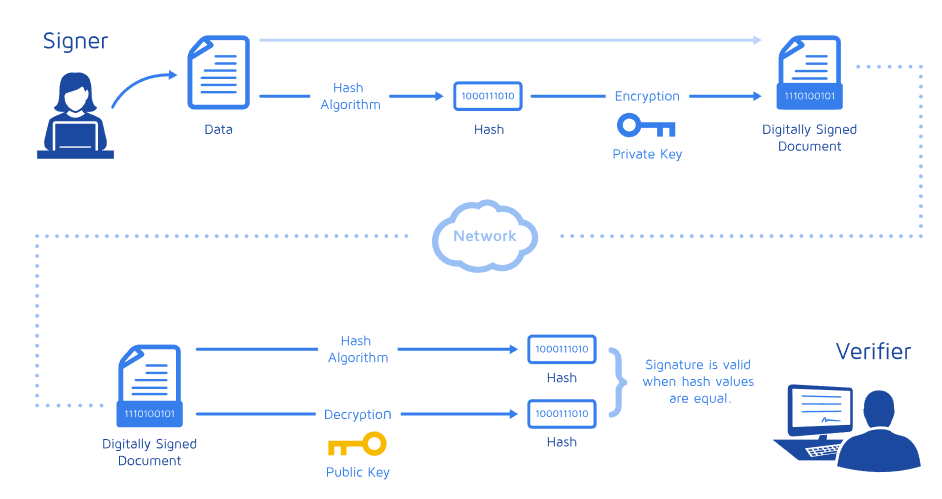
\includegraphics[scale=0.5]{key}

\subsection{Advantages and Disadvantages of Digital Signature}
Advantages of digital signature:
\begin{enumerate}
  \item A digital signature provides better security in the transaction. Any unauthorized person cannot do fraudulence in transactions.
  \item You can easily track the status of the documents on which the digital signature is applied.
  \item High speed up document delivery.
  \item It is 100\% legal it is issued by the government authorized certifying authority.
  \item If you have signed a document digitally, then you cannot deny it.
  \item In this signature, When a document is get signed, date and time are automatically stamped on it.
\end{enumerate}
Disadvantages of Digital Signature:*****
\begin{enumerate}
\item Criminals can create fraudulent websites that appear to be yours, they can create malware that purports to be software originating from you, and they steal credit card details and other valuable information that customers believe only you can decrypt.
\item Software is one of the main issues while using a digital signature certificate.
\item In this signature, Lost or theft of keys and the use of vulnerable storage facilities.
\item There is a stronger need for a standard through which these different methods can interact.
\item To work with digital certificates, the sender and recipients have to buy verification software at a cost.
\end{enumerate}
\section{Privacy issues of information management system}
Privacy and security are problems associated with computer systems and applications that were not foreseen until well into the second half of the present computer age. Privacy is an issue that concerns the computer community in connection with maintaining personal information on individual citizens in computerized record-keeping systems. It deals with the rights of the individual regarding the collection information in a record-keeping system about his person and activities, and the processing, dissemination, storage, and use of this information in making determinations about him.
\begin{enumerate}
  \item Emberdding data privacy

    There is a broad lack of information and understanding about embedded data, where it resides, and the financial and reputational risk it poses to businesses.
  \item Proliferating devices

    Data privacy becomes harder to handle when you factor in things like the Internet of Things (IOT), bring-your-own-device IT policies and proliferating internet-connected tablets, phones and watches.
  \item Increasing maintenance consts
    Keeping your systems secure and preventing data privacy issues at the enterprise level can be expensive. But, the costs of a data breach are so significant, you need to bite the bullet and invest properly.
  \item Access control is difficult in many industries

    Data privacy breaches are often caused by poorly managed access within an organization. People and processes matter as much as technology. Humans are the weakest link in the chain of privacy and security.
  \item Getting visibility into all your data

    Using tools to discover and classify your data is essential. This will ensure you can treat data uniquely and protect your sensitive data from any privacy issues.
  \item A bad data culture

    Today, keeping data for its own sake broadens the attack surface for data theft and increases the risk of breaching many data privacy laws. Forward-thinking IT teams need to balance the value of collecting, storing and processing large volumes of data against the pressing requirements for privacy, security and compliance.
  \item The ever-incresing scale of data

    With hundreds of systems and millions of data records, we need a solution that can handle the scale.
  \item A long list of regulations and documentation to follow

    With so many regulations to follow, it can be difficult to keep track of what level of data privacy you need to achieve for your different datasets.
\end{enumerate}
\section{Cyber Crime/Computer Crime}
Cyber-crime refers to the use of information technology to commit crimes. Cyber-crimes can range from simply annoying computer users to huge financial losses and even the loss of human life. The growth of smartphones and other high-end Mobile devices that have access to the internet have also contributed to the growth of cyber-crime.

Types of cyber-crime:
\begin{enumerate}
  \item Identity theft
  \item Copyright infringement
  \item Click fraud
  \item Advance Fee Fraud
  \item Hacking
  \item Computer virus
\end{enumerate}

\section{How to prevent computer crime?\\or\\Major concerns about computer crime and privacy, and how to protect/prevent them?}
There are different major concerns about computer crime and privacy on the internet which refers to criminal conduct committed with the aid of a computer or other electronic equipment connected to the internet. Individuals or small groups of people with little technical knowledge and highly organized worldwide criminal groups with relatively talented developers and specialists can engage in cybercrime.

For example:
\begin{enumerate}
  \item Stolen credit card information: The most common cybercrime is when a person’s credit card information is stolen and used unlawfully to acquire or purchase goods or services over the internet.
  \item Hacking into a government website: Another type of cybercrime is tampering with sensitive government data.
  \item Theft of user accounts: Yahoo experienced a serious data breach from 2013 to 2016  that resulted in the theft of three billion user accounts. The attackers gained access to private information and passwords that were used to access user accounts in other online services. Most of this data is available even today on the dark web.
  \item Compromised IoT devices: In 2016, over one million connected devices in the IoT were compromised by attackers who took advantage of existing software vulnerabilities. It is the largest DDoS attack to date.
  \item Loss of control and access to content: The WannaCry attack, which was allegedly launched by North Korea, in 2017, unleashed ransomware that locked down content on user devices. This ransomware rapidly spread itself and infected 300,000 computers worldwide.
\end{enumerate}
\subsection{How to protect ourrself against cybercrime?}
Anyone using the internet should exercise some basic precautions as follows

\begin{enumerate}
  \item Use a full-service internet security suite: 

It’s a good idea to consider trusted security software that provides all-in-one protection for your devices, online privacy, and identity and helps protect your private and financial information when you go online.
\item Use strong passwords: 

Don’t repeat passwords on different sites, and change your passwords regularly. Make them complex. That means using a combination of at least 10 letters, numbers, and symbols.
\item Keep your software updated: 

This is especially important with your operating systems and internet security software. Cybercriminals frequently use known exploits, or flaws, in your software to gain access to your system.
\item Manage your social media settings: 

Keep your personal and private information locked down. Social engineering cybercriminals can often get your personal information with just a few data points.
\item Strengthen your home network:


It’s a good idea to start with a strong encryption password as well as a virtual private network. A VPN will encrypt all traffic leaving your devices until it arrives at its destination.
\item Keep up to date on major security breaches:

If you do business with a merchant or have an account on a website that’s been impacted by a security breach, find out what information the hackers accessed and change your password immediately.

\item Take measures to help protect yourself against identity theft:

Identity theft occurs when someone wrongfully obtains your personal data in a way that involves fraud or deception, typically for economic gain.
\end{enumerate}

\part{Unit 5}
\section{Procurement Management System}
Procurement management is responsible for overseeing all the processes involved in acquiring the products, materials, goods and services needed for efficient business operations. Depending on the business and industry, the terms “sourcing,” “purchasing” and “procurement” may be used interchangeably to describe the function of procuring supplies and managing the process, with sourcing considered more strategic, and purchasing and procurement used to refer to the actual operational function.
\subsection{What are the Steps of the Procurement Process?}
\begin{enumerate}
  \item [\textbf{Step 1:}] Specifying and Planning
  \item [\textbf{Step 2:}] Identifying and Selecting Suppliers
  \item [\textbf{Step 3:}] Negotiating and Contracting
  \item [\textbf{Step 4:}] Placing the Purchase Order
  \item [\textbf{Step 5:}] Expediting
  \item [\textbf{Step 6:}] Receipt and Inspection of Purchase
  \item [\textbf{Step 7:}] Invoice Clearing and Payment
  \item [\textbf{Step 8:}] Maintaining Records and Relationships
\end{enumerate}

\section{ERP System works in an organizations like Amazon/Flipkart/Snapdeal}
ERP systems work via a central database. Users look at dashboards to view real-time data across different business units such as sales, supply chain management, and personnel.

ERP is an integrated system of software applications that allows an organization to manage its business processes using a centralized relational database. It allows a business to see a snapshot of how efficiently its key functions, for example, inventory levels or sales, and personnel are working together.

ERP systems typically contain dashboards connected to a central database that let users look at real-time data across different business units.

\begin{figure}[h]
  \centering
  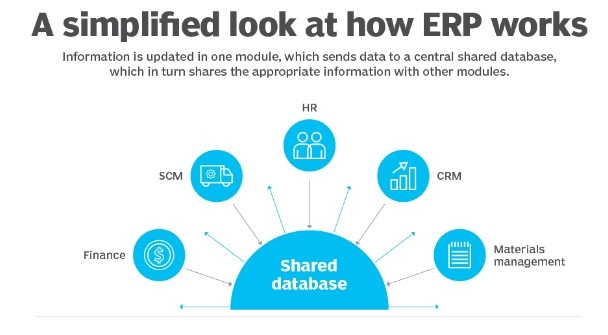
\includegraphics[scale=0.4]{howerpworks}
  \caption{A simplified look at how ERP works in Amazon/Flipkart/Snapdeal}
\end{figure}
In an ERP system, information is uploaded in one module and shared to the central database, which shares the information with other modules.

\begin{figure}[h]
  \centering
  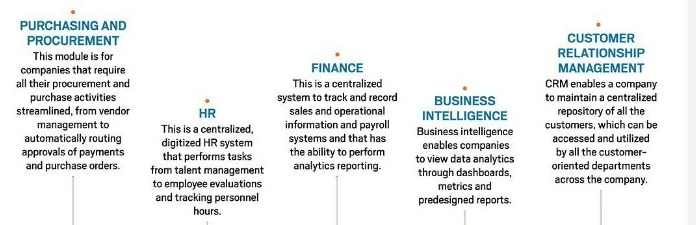
\includegraphics[scale=0.5]{erpcomp}
  \caption{Different ERP components used in different organizations like Amazon/ Flipkart}
\end{figure}

Amazon / Flipkart basically perform Online sales i.e  also known as e-commerce, the online sales module allows customers to see changes in prices, catalog, inventory and the supply chain, and have those changes reflected in customer-facing messaging. ERP vendors offer e-commerce applications for all sales channels, whether B2B, B2C or C2C. Ideally, this module allows us to manage both consumer and wholesale channels on a single platform. Online sales ERP applications can also let retail or wholesale partners update product information on their end.


\end{document}
